\documentclass[11 pt]{article}
	\usepackage{beppe_package}
	\usepackage[a4paper, left=2.5cm, right=2.5cm, bottom=2.5cm]{geometry}
	
	\newcommand{\ai}{\mathrm{Ai}}
	\newcommand{\bi}{\mathrm{Bi}}
	\renewcommand{\S}{\mathcal{S}}
	\renewcommand{\Re}{\mathrm{Re}}
	\renewcommand{\Im}{\mathrm{Im}}
	
	\title{Funzioni di Airy}
	\author{Giuseppe Bogna}
	\date{\today}
	
\begin{document}
	\maketitle
	\section*{Introduzione}
	Le funzioni di Airy $\ai$ e $\bi$ sono le funzioni di una variabile reale $x$
	\begin{align}
		\ai(x)&=\frac{1}{\pi}\int_{0}^{+\infty}\cos\left(xt+\frac{t^3}{3}\right)\d t\label{eq:airy1}\\\bi(x)&=\frac{1}{\pi}\int_{0}^{+\infty}\left[\exp\left(-\frac{t^3}{3}+xt\right)+\sin\left(xt+\frac{t^3}{3}\right)\right]\d t\label{eq:airy2}
	\end{align}
	e hanno notevoli applicazioni in fisica. Storicamente, la prima funzione di Airy $\ai$ è stata introdotta (ma guarda un po') da Airy, come soluzione dell'equazione
	\begin{equation}y''-xy=0\label{eq:ode}\end{equation}
	La seconda funzione di Airy $\bi$ viene introdotta per costruire tutte le possibili soluzioni di \ref{eq:ode}. 
	\section{Buona definizione delle funzioni di Airy}
	Cominciamo col mostrare che gli integrali \ref{eq:airy1} e \ref{eq:airy2} convergono. Ad esempio, mostriamo che per ogni $x$ esiste finito
	\[L_x=\lim\limits_{z\to+\infty}\int_{0}^{z}\cos\left(xt+\frac{t^3}{3}\right)\d t\]
	Sia $g_x(t)=xt+t^3/3$. Ovviamente per ogni $x$ esiste $\tau_x>0$ tale che $g_x$ sia invertibile per $t\in(\tau_x,+\infty)$. Posto $\xi=g_x(t)$, supponiamo di conoscere la funzione inversa $t_x(\xi)$. Allora è
	\[\int_{0}^{z}\cos\left(xt+\frac{t^3}{3}\right)\d t=\int_{0}^{\tau_x}\cos\left(xt+\frac{t^3}{3}\right)\d t+\int_{\tau_x}^{z}\frac{\cos\xi}{x+t^2_x(\xi)}\d \xi\]
	Il primo integrale a secondo membro converge, quindi concentriamoci sul secondo. Chiamiamolo per brevità $I_x$. Se $x\geq0$ questo ha problemi di convergenza solo a $+\infty$, quindi possiamo limitarci a considerare l'andamento per grandi $\xi$ della funzione integranda. Per grandi $\xi$ chiaramente $t_x(\xi)\simeq\sqrt[3]{3\xi}$, dunque integrando per parti
	\[I_{x}\simeq\int_{\tau_x}^{z}\frac{\cos\xi}{(3\xi)^{2/3}}\d \xi=\left.\frac{\sin\xi}{(3\xi)^{2/3}}\right|_{\tau_x}^{z}+\frac{2}{3\sqrt[3]{9}}\int_{\tau_x}^{z}\frac{\sin\xi}{\xi^{5/3}}\d \xi\]
	L'ultimo integrale converge, dato che
	\[\left|\int_{\tau_x}^{z}\frac{\sin\xi}{\xi^{5/3}}\d \xi\right|\leq\int_{\tau_x}^{z}\frac{1}{\xi^{5/3}}\d \xi\]
	e quest'ultimo integrale esiste finito per $z\to+\infty$. Il termine di bordo dipendente da $z$ ottenuto nell'integrazione per parti si annulla quando $z\to+\infty$, quindi $L_x$ esiste finito. Se invece $x<0$, basta scegliere $\tau_x$ sufficientemente grande in modo che $t_x(\xi)>\sqrt{x}$ se $\xi>\tau_x$, in modo da eliminare un eventuale zero del denominatore. In conclusione $L_x$ converge per ogni $x$ e $\ai$ è ben definita. Per $\bi$ si ha una trattazione analoga per la parte con il seno, mentre la parte esponenziale non ha chiaramente problemi di convergenza.
	\section{Derivazione della prima funzione di Airy}
	Cerchiamo soluzioni $\S'$ della \ref{eq:ode} tramite trasformata di Fourier. Usiamo per la trasformata la convenzione
	\[\hat{f}(k)=\int_{-\infty}^{+\infty}f(x)e^{-ikx}\d x\]
	In questo modo si ha
	\[\hat{f}^{(n)}(k)=(-i)^n\int_{-\infty}^{+\infty}x^nf(x)e^{-ikx}\d x,\qquad\qquad k^n\hat{f}(k)=(-i)^n\int_{-\infty}^{+\infty}f^{(n)}(x)e^{-ikx}\d x\]
	Trasformando la \ref{eq:ode} si ottiene allora
	\begin{equation}k^2\hat{f}+i\hat{f}'=0\label{eq:odeft}\end{equation}
	La soluzione è, a meno di una costante moltiplicativa,
	\[\hat{f}(k)=e^{ik^3/3}\]
	Quindi si ha
	\[f(x)=\frac{1}{2\pi}\int_{-\infty}^{+\infty}e^{ik^3/3+ikx}\d k\]
	Questa è proprio $\ai$, come si vede scrivendo l'esponenziale in termini di seni e coseni e usando le proprietà di parità di tali funzioni. Si noti che la soluzione ottenuta è in $\S'$, ma non in $\mathbb{L}^2(\R)$.\footnote{Infatti $\hat{f}$ non è ovviamente in $\mathbb{L}^2(\R)$, mentre la trasformata di Fourier di una funzione in $\mathbb{L}^2(\R)$ è ancora in $\mathbb{L}^2(\R)$.} Inoltre, abbiamo ottenuto una sola soluzione: l'altra, come vedremo, diverge esponenzialmente a $+\infty$, quindi non può essere ottenuta con le trasformate. Ciò è in realtà intuibile dal fatto che, trasformando, siamo passati dall'equazione \ref{eq:ode}, del secondo ordine, all'equazione \ref{eq:odeft}, del primo ordine.
	\section{Derivazione della seconda funzione di Airy}
	Cerchiamo di generalizzare quanto appena fatto. Supponiamo di poter scrivere una soluzione di \ref{eq:ode} nella forma
	\[y(x)=\int_{\Gamma}u(z)e^{ixz}\d z\]
	dove $\Gamma$ è un cammino opportuno nel piano complesso e $u$ un'opportuna funzione. L'obiettivo è determinare sia $u$ che $\Gamma$. Supponendo di poter derivare sotto il segno di integrale, vogliamo che sia
	\[y''(x)-xy(x)=-\int_{\Gamma}(z^2+x)u(z)e^{ixz}=0\]
	Integrando per parti si deduce
	\[\int_{\Gamma}(z^2+x)u(z)e^{ixz}=\left.-iu(z)e^{ixz}\right|_{\partial\Gamma}+\int_{\Gamma}(z^2u(z)+iu'(z))e^{ixz}\d z\]
	Poniamo $u(z)=\exp(iz^3/3)$, in modo da annullare l'integrale a secondo membro qualunque sia il percorso di integrazione\footnote{Questa scelta rende anche lecita la derivazione sotto il segno di integrale.}. Fatto questo, scegliamo $\Gamma$ in modo che $u(z)e^{ixz}$ si annulli agli estremi del contorno. Vediamo se è possibile cercare un percorso $\Gamma$ che vada all'infinito. Posto $z=\rho e^{i\theta}$, si ha
	\[u(z)e^{izx}=\exp\left(i\rho^3\cos3\theta-\rho^3\sin3\theta+i\rho x\cos\theta-\rho x\sin\theta\right)\]
	dunque $\Gamma$ ha la proprietà richiesta se asintoticamente si trova in una regione in cui $\sin3\theta>0$. Questo corrisponde alle regioni $0<\arg z<\pi/3$, $2\pi/3<\arg z<\pi$ e $4\pi/3<\arg z<5\pi/3$, ossia nelle regioni non ombreggiate in figura \ref{fig:admreg}.
	\begin{figure}[h!]
		\centering
		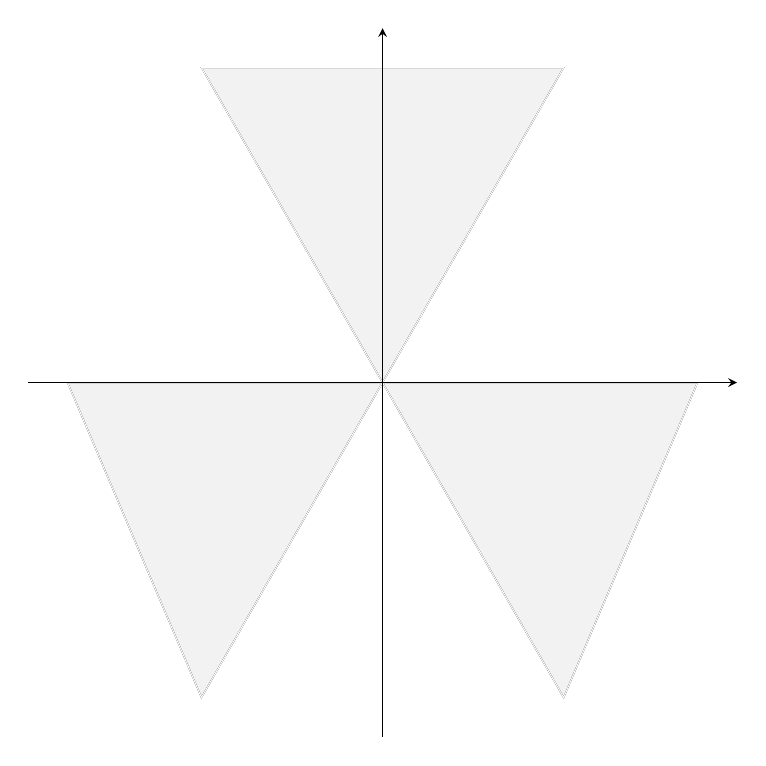
\begin{tikzpicture}
		\draw [fill=gray!10](0,0)--(2.3,4)--(-2.3,4)--(0,0);
		\draw [white](0,0)--(2.3,4)--(-2.3,4)--(0,0);
		\draw [fill=gray!10](0,0)--(-4,0)--(-2.3,-4)--(0,0);
		\draw [white](0,0)--(-4,0)--(-2.3,-4)--(0,0);
		\draw [fill=gray!10](0,0)--(4,0)--(2.3,-4)--(0,0);
		\draw [white](0,0)--(4,0)--(2.3,-4)--(0,0);
		\draw [-stealth](0,-4.5)--(0,4.5);
		\draw [-stealth](-4.5,0)--(4.5,0);
		
		\end{tikzpicture}
		\caption{regioni asintotiche permesse per $\Gamma$.}
		\label{fig:admreg}
	\end{figure}

	\noindent Chiaramente, per come abbiamo costruito la soluzione possiamo considerare anche funzioni della forma
	\[f(x)=\int_{\Gamma_1}e^{iz^3/3+ixz}\d z+\int_{\Gamma_2}e^{iz^3/3+ixz}\d z\]
	con $\Gamma_1$ e $\Gamma_2$ percorsi che rispettano le condizioni date.
	
	Prendiamo adesso come $\Gamma_1$ il semiasse immaginario negativo, percorso verso lo zero, unito al semiasse reale negativo, percorso allontanandosi dallo zero; come $\Gamma_2$ prendiamo sempre il semiasse immaginario negativo, percorso verso lo zero, unito però al semiasse reale positivo, percorso allontanandosi dallo zero. In linea di principio non abbiamo garanzie sulla convergenza della funzione ottenuta, a causa dei tratti con $\arg z=0$ e $\arg z=\pi$, tuttavia la funzione così ottenuta coincide, a meno di una costante moltiplicativa, con $\bi$, che converge. Alternativamente, potremmo anche sostituire i tratti sull'asse reale con tratti del tipo $\xi+i\varepsilon$ e poi fare il limite $\varepsilon\to0$. Mostriamo quanto appena detto:
	\begin{align*}
		\int_{\Gamma_1}e^{iz^3/3+ixz}\d z&=i\int_{-\infty}^{0}e^{t^3/3-xt}\d t-\int_{0}^{+\infty}e^{-it^3/3-ixt}\d t=\\&=\int_{0}^{+\infty}\left(ie^{-t^3/3+xt}-e^{-it^3/3+ixt}\right)\d t\\
		\int_{\Gamma_2}e^{iz^3/3+ixz}\d z&=i\int_{-\infty}^{0}e^{t^3/3-xt}\d t+\int_{0}^{+\infty}e^{it^3/3+ixt}\d t=\\&=\int_{0}^{+\infty}\left(ie^{-t^3/3+xt}+e^{it^3/3+ixt}\right)\d t
	\end{align*}
	Dunque
	\begin{align*}		
		\int_{\Gamma_1}e^{iz^3/3+ixz}\d z+\int_{\Gamma_2}e^{iz^3/3+ixz}\d z&=2i\int_{0}^{+\infty}e^{-t^3/3+xt}\d t+\int_{0}^{+\infty}\left(e^{it^3/3+ixt}+e^{-t^3/3-ixt}\right)\d t=\\&=2\pi i\bi(x)
	\end{align*}
	\section{Ortogonalità}
	Sia $\ai_x$ la traslazione di $x$ della prima funzione di Airy, ossia
	\[\ai_x(t)=\ai(t-x)\]
	Si mostra facilmente che $\left\{\ai_x\right\}_{x\in\R}$ è un insieme ortonormale, nel senso delle distribuzioni. Infatti usando la rappresentazione integrale della $\delta$ di Dirac
	\begin{align*}
		\int_{-\infty}^{+\infty}\ai_x(t)\ai_y(t)\d t&=\frac{1}{4\pi ^2}\int_{-\infty}^{+\infty}\d t\int_{-\infty}^{+\infty}\d\sigma\exp\left[i(t-x)\sigma+i\frac{\sigma^3}{3}\right]\int_{-\infty}^{+\infty}\d\omega\exp\left[i(t-y)\omega+i\frac{\omega^3}{3}\right]=\\&=\frac{1}{4\pi^2}\int_{-\infty}^{+\infty}\d\sigma\exp\left(-ix\sigma+i\frac{\sigma^3}{3}\right)\int_{-\infty}^{+\infty}\d\omega\exp\left(-iy\omega+i\frac{\omega^3}{3}\right)\int_{-\infty}^{+\infty}\d t\exp\left(it\sigma+it\omega\right)=\\&=\frac{1}{2\pi}\int_{-\infty}^{+\infty}\d\sigma\exp\left(-ix\sigma+i\frac{\sigma^3}{3}\right)\int_{-\infty}^{+\infty}\d\omega\exp\left(-iy\omega+i\frac{\omega^3}{3}\right)\delta(\omega+\sigma)=\\&=\frac{1}{2\pi}\int_{-\infty}^{+\infty}\d\sigma\exp(i\sigma y-i\sigma x)=\\&=\delta(x-y)
	\end{align*}
	\section{Andamenti asintotici}
	Usiamo il metodo del punto sella per stimare le due funzioni di Airy quando $|x|$ è grande. Ricordiamo brevemente che se si ha un integrale della forma
	\[I=\int_{\gamma}f(z)e^{\lambda g(z)}\d z\]
	e lo si vuole stimare per grandi valori di $\lambda$, si può deformare $\gamma$ in modo che 
	\begin{itemize}
		\item $\gamma$ passi per un punto $z_0$ in cui $g'(z_0)=0$,
		\item $\Re g$ abbia un massimo vincolato su $\gamma$ in $z_0$,
		\item $\Im g$ sia costante in un qualche intorno di $z_0$ ristretto a $\gamma$.
	\end{itemize}
	Per semplicità supponiamo anche che $f(z_0)\neq0$ e $g''(z_0)\neq0$. Sotto tali ipotesi, se il vettore tangente a $\gamma$ in $z_0$ è $e^{i\alpha}$ si ha
	\[I\simeq\sqrt{\frac{2\pi}{\lambda|g''(z_0)|}}f(z_0)e^{\lambda g(z_0)+i\alpha}\]
	Per i nostri scopi, possiamo cercare i punti in cui la parte immaginaria degli esponenti degli esponenziali è stazionaria e espandere al secondo ordine in tali punti.
	Vediamo adesso gli sviluppi asintotici.
	
	Per $\ai$ conviene usare la forma
	\[\ai(x)=\frac{1}{2\pi}\int_{-\infty}^{+\infty}e^{ixt+it^3/3}\d t\]
	Supponiamo ora $x<0$. La fase è stazionaria per	$t=\pm\sqrt{|x|}$. In tali punti la derivata seconda è $\pm2i\sqrt{|x|}$, dunque si ottiene
	\begin{align*}
		\ai(x)&\simeq\frac{1}{2\pi}\int_{-\infty}^{+\infty}\left[\exp\left(-\frac{2}{3}i|x|^{3/2}+i\sqrt{|x|}(t-\sqrt{|x|})^2\right)+\exp\left(\frac{2}{3}i|x|^{3/2}-i\sqrt{|x|}(t-\sqrt{|x|})^2\right)\right]\d t=\\&=\frac{1}{\sqrt{\pi}|x|^{1/4}}\cos\left(\frac{2}{3}|x|^{3/2}-\frac{\pi}{4}\right)
	\end{align*}
	Si è usato in particolare il fatto che per $\alpha$ reale
	\[\int_{-\infty}^{+\infty}e^{i\alpha \xi^2}\d \xi=\sqrt{\frac{\pi}{|\alpha|}}e^{i\frac{\pi}{4}\textrm{sgn}\alpha}\]
	Supponiamo ora $x>0$. Questa volta la fase è stazionaria per $t=\pm i\sqrt{x}$, che \textit{non} appartengono al cammino su cui integriamo. La derivata seconda in tali punti è $\mp\sqrt{x}$. Deformiamo quindi l'asse reale in modo tale che passi solo per $i\sqrt{x}$, con vettore tangente puramente reale. Si noti ora che dobbiamo integrare una gaussiana che ha larghezza $1/\sqrt{x}$. Dato che $x$ è grande, le code della gaussiana diventano piccole già molto vicino al valor medio, quindi possiamo estendere l'integrale a tutta la retta senza compiere particolari errori. Si ottiene così
	\begin{align*}
		\ai(x)&\frac{1}{2\pi}\simeq\int_{-\infty}^{+\infty}\exp\left(-\frac{2}{3}x^{3/2}-\sqrt{x}(t-i\sqrt{x})^2\right)\d t=\\&=\frac{1}{2\sqrt{\pi}x^{1/4}}e^{-\frac{2}{3}x^{3/2}}	
	\end{align*}
	dove si è usato il fatto che per $\alpha$ reale positivo e $\beta$ complesso
	\[\int_{-\infty}^{+\infty}e^{-\alpha x^2+i\beta x}\d x=\sqrt{\frac{\pi}{\alpha}}e^{-\beta^2/4\alpha}\]
	
	Passiamo a $\bi$ e trattiamo separatamente la parte con il seno e la parte esponenziale. Per la prima, scriviamo
	\[\int_{0}^{+\infty}\sin\left(xt+\frac{t^3}{3}\right)\d t=\Im\int_{0}^{+\infty}e^{ixt+it^3/3}\d t\]
	Come nel caso precedente, per $x<0$ la fase è stazionaria per $t=\pm\sqrt{|x|}$. Solo il primo punto è nel cammino di integrazione, dunque
	\begin{align*}
		\int_{0}^{+\infty}\sin\left(xt+\frac{t^3}{3}\right)\d t&\simeq\Im\int_{0}^{+\infty}\exp\left(-\frac{2}{3}i|x|^{3/2}+i\sqrt{|x|}(t-\sqrt{|x|})^2\right)\d t\simeq\\&\simeq
		\Im\int_{-\infty}^{+\infty}\exp\left(-\frac{2}{3}i|x|^{3/2}+i\sqrt{|x|}(t-\sqrt{|x|})^2\right)\d t=\\&=\frac{\sqrt{\pi}}{|x|^{1/4}}\sin\left(\frac{\pi}{4}-\frac{2}{3}|x|^{3/2}\right)=\\&=\frac{\sqrt{\pi}}{|x|^{1/4}}\cos\left(\frac{2}{3}|x|^{3/2}+\frac{\pi}{4}\right)
	\end{align*} 
	Per $x>0$ la fase è stazionaria per $t=\pm i\sqrt{x}$. Deformiamo il contorno di integrazione in modo da passare solo per il primo punto, così
	\begin{align*}
	\int_{0}^{+\infty}\sin\left(xt+\frac{t^3}{3}\right)\d t&\simeq
	\Im\int_{-\infty}^{+\infty}\exp\left(-\frac{2}{3}x^{3/2}-\sqrt{x}(t-i\sqrt{x})^2\right)\d t=\\&=0
	\end{align*} 
	Passiamo alla parte esponenziale. Per $x<0$ abbiamo la stima
	\begin{align*}0\leq\int_{0}^{+\infty}e^{xt-t^3/3}\d t&=\left.\frac{e^{xt-t^3/3}}{x}\right|_0^{+\infty}+\frac{1}{x}\int_{0}^{+\infty}t^2e^{xt+t^3/3}\d t=\\&=\frac{1}{x}\left(1+\int_{0}^{+\infty}t^2e^{xt+t^3/3}\d t\right)\leq\\&=\frac{1}{x}\left(1+\int_{0}^{+\infty}t^2e^{-t^3/3}\d t\right)=\frac{\alpha}{x}\end{align*}
	quindi il contributo dell'esponenziale è trascurabile rispetto a quello del seno. Per $x>0$ invece i punti a fase stazionaria sono $t=\pm\sqrt{x}$ e solo il primo si trova sul percorso di integrazione. Allora
	\begin{align*}
		\int_{0}^{+\infty}e^{xt-t^3/3}\d t&\simeq\int_{-\infty}^{+\infty}e^{\frac{2}{3}x^{3/2}-\sqrt{x}(t-\sqrt{x})^2}\d t=\\&=\frac{\sqrt{\pi}}{x^{1/4}}e^{\frac{2}{3}x^{3/2}}
	\end{align*}
	Unendo tutti questi risultati e riprendendo quelli su $\ai$ abbiamo quindi
	\begin{align*}
		\ai(x)&\simeq\begin{cases}\dfrac{1}{\sqrt{\pi}|x|^{1/4}}\cos\left(\dfrac{2}{3}|x|^{3/2}-\dfrac{\pi}{4}\right)&\textrm{ per }x\to-\infty\\[10pt]\dfrac{1}{2\sqrt{\pi}x^{1/4}}e^{-\frac{2}{3}x^{3/2}}&\textrm{ per }x\to+\infty
		\end{cases}\\
		\bi(x)&\simeq\begin{cases}\dfrac{1}{\sqrt{\pi}|x|^{1/4}}\cos\left(\dfrac{2}{3}|x|^{3/2}+\dfrac{\pi}{4}\right)&\textrm{ per }x\to-\infty\\[10pt]\dfrac{1}{2\sqrt{\pi}x^{1/4}}e^{\frac{2}{3}x^{3/2}}&\textrm{ per }x\to+\infty
		\end{cases}
	\end{align*}
\end{document}